\documentclass{article}

% ---------------------------------------------------------------- %
% short package descriptions are copied from
% https://ctan.org/

% ---------------------------------------------------------------- %

% Accept different input encodings
\usepackage[utf8]{inputenc}

% Standard package for selecting font encodings
\usepackage[T1]{fontenc}

% ---------------------------------------------------------------- %

% Multilingual support for Plain TEX or LATEX
\usepackage[english]{babel}

% ---------------------------------------------------------------- %

% Set all page margins to 1.5cm
\usepackage{fullpage}

% Margin adjustment and detection of odd/even pages
\usepackage{changepage}

% Flexible and complete interface to document dimensions
\usepackage{geometry}

% ---------------------------------------------------------------- %
% mathematics

\usepackage{amsmath}  % AMS mathematical facilities for LATEX
\usepackage{amssymb}
\usepackage{amsfonts} % TEX fonts from the American Mathematical Society
\usepackage{amsthm}   % Typesetting theorems (AMS style)

% Mathematical tools to use with amsmath
\usepackage{mathtools}

% Support for using RSFS fonts in maths
\usepackage{mathrsfs}

% Commands to produce dots in math that respect font size
\usepackage{mathdots}

% "Blackboard-style" cm fonts
\usepackage{bbm}

% Typeset in-line fractions in a "nice" way
\usepackage{nicefrac}

% Typeset quotient structures with LATEX
\usepackage{faktor}

% Vector arrows
\usepackage{esvect}

% St Mary Road symbols for theoretical computer science
\usepackage{stmaryrd}

% Three series of mathematical symbols
\usepackage{mathabx}

% ---------------------------------------------------------------- %
% algorithms

% Package for typesetting pseudocode
\usepackage{algpseudocode}

% Typeset source code listings using LATEX
\usepackage{listings}

% Reimplementation of and extensions to LATEX verbatim
\usepackage{verbatim}

% If necessary, please use the following 2 packages locally, but never both.
% This is because the algorithm environment gets defined in both packages, which leads to name conflicts.
% \usepackage{algorithm2e}
% \usepackage{algorithm}

% ---------------------------------------------------------------- %
% utilities

% A generic document command parser
\usepackage{xparse}

% Extended conditional commands
\usepackage{xifthen}

% e-TEX tools for LATEX
\usepackage{etoolbox}

% Define commands with suffixes
\usepackage{suffix}

% Extensive support for hypertext in LATEX
\usepackage{hyperref}

% Driver-independent color extensions for LATEX and pdfLATEX
\usepackage{xcolor}

% ---------------------------------------------------------------- %
% graphics

% -------------------------------- %

\usepackage{tikz}

% MISC
\usetikzlibrary{patterns}
\usetikzlibrary{decorations.markings}
\usetikzlibrary{positioning}
\usetikzlibrary{arrows}
\usetikzlibrary{arrows.meta}
\usetikzlibrary{overlay-beamer-styles}

% finite state machines
\usetikzlibrary{automata}

% turing machines
\usetikzlibrary{calc}
\usetikzlibrary{chains}
\usetikzlibrary{decorations.pathmorphing}

% -------------------------------- %

% Draw tree structures
\usepackage[noeepic]{qtree}

% Enhanced support for graphics
\usepackage{graphicx}

% Figures broken into subfigures
\usepackage{subfig}

% Improved interface for floating objects
\usepackage{float}

% Control float placement
\usepackage{placeins}

% Include PDF documents in LATEX
\usepackage{pdfpages}

% ---------------------------------------------------------------- %

% Control layout of itemize, enumerate, description
\usepackage[inline]{enumitem}

% Intermix single and multiple columns
\usepackage{multicol}
\setlength{\columnsep}{1cm}

% Coloured boxes, for LATEX examples and theorems, etc
\usepackage{tcolorbox}

% ---------------------------------------------------------------- %
% tables

% Tabulars with adjustable-width columns
\usepackage{tabularx}

% Tabular column heads and multilined cells
\usepackage{makecell}

% Publication quality tables in LATEX
\usepackage{booktabs}

% ---------------------------------------------------------------- %
% bibliography and quoting

% Sophisticated Bibliographies in LATEX
\usepackage[backend = biber, style = alphabetic]{biblatex}

% Context sensitive quotation facilities
\usepackage{csquotes}

% ---------------------------------------------------------------- %

% ---------------------------------------------------------------- %
% special letters

\newcommand{\N}{\mathbb N}
\newcommand{\Z}{\mathbb Z}
\newcommand{\Q}{\mathbb Q}
\newcommand{\R}{\mathbb R}
\newcommand{\C}{\mathbb C}
\newcommand{\K}{\mathbb K}
\newcommand{\T}{\mathbb T}
\newcommand{\E}{\mathbb E}
\newcommand{\V}{\mathbb V}
\renewcommand{\S}{\mathbb S}
\renewcommand{\P}{\mathbb P}
\newcommand{\1}{\mathbbm 1}
\newcommand{\G}{\mathbb G}

\newcommand{\iu}{\mathrm i}

% ---------------------------------------------------------------- %
% quantors

\newcommand{\Forall}        {\forall \,}
\newcommand{\Exists}        {\exists \,}
\newcommand{\nExists}       {\nexists \,}
\newcommand{\ExistsOnlyOne} {\exists! \,}
\newcommand{\nExistsOnlyOne}{\nexists! \,}
\newcommand{\ForAlmostAll}  {\forall^\infty \,}

% ---------------------------------------------------------------- %
% graphics boxed

\newcommand
{\includegraphicsboxed}
[2][0.75]
{
  \begin{center}
    \begin{tcolorbox}[standard jigsaw, opacityback = 0]

      \centering
      \includegraphics[width = #1 \textwidth]{#2}

    \end{tcolorbox}
  \end{center}
}

\newcommand
{\includegraphicsunboxed}
[2][0.75]
{
  \begin{center}
    \includegraphics[width = #1 \textwidth]{#2}
  \end{center}
}

\NewDocumentCommand
{\includegraphicsgraphicsboxed}
{ O{0.75} O{0.25} m m}
{
  \begin{center}
    \begin{tcolorbox}[standard jigsaw, opacityback = 0]

      \centering
      \includegraphics[width = #1 \textwidth]{#3} \\
      \vspace{#2 cm}
      \includegraphics[width = #1 \textwidth]{#4}

    \end{tcolorbox}
  \end{center}
}

\NewDocumentCommand
{\includegraphicsgraphicsunboxed}
{ O{0.75} O{0.25} m m}
{
  \begin{center}

    \centering
    \includegraphics[width = #1 \textwidth]{#3} \\
    \vspace{#2 cm}
    \includegraphics[width = #1 \textwidth]{#4}

  \end{center}
}

% ---------------------------------------------------------------- %
% braces

\newcommand{\pbraces}[1]{{\left  ( #1 \right  )}}
\newcommand{\bbraces}[1]{{\left  [ #1 \right  ]}}
\newcommand{\Bbraces}[1]{{\left \{ #1 \right \}}}
\newcommand{\vbraces}[1]{{\left  | #1 \right  |}}
\newcommand{\Vbraces}[1]{{\left \| #1 \right \|}}

\newcommand{\abraces}[1]{{\left \langle #1 \right \rangle}}

\newcommand{\floorbraces}[1]{{\left \lfloor #1 \right \rfloor}}
\newcommand{\ceilbraces} [1]{{\left \lceil  #1 \right \rceil }}

\newcommand{\dbbraces}    [1]{{\llbracket     #1 \rrbracket}}
\newcommand{\dpbraces}    [1]{{\llparenthesis #1 \rrparenthesis}}
\newcommand{\dfloorbraces}[1]{{\llfloor       #1 \rrfloor}}
\newcommand{\dceilbraces} [1]{{\llceil        #1 \rrceil}}

\newcommand{\dabraces}[1]{{\left \langle \left \langle #1 \right \rangle \right \rangle}}

\newcommand{\abs}  [1]{\vbraces{#1}}
\newcommand{\round}[1]{\bbraces{#1}}
\newcommand{\floor}[1]{\floorbraces{#1}}
\newcommand{\ceil} [1]{\ceilbraces{#1}}

% ---------------------------------------------------------------- %

% MISC

% metric spaces
\newcommand{\norm}[2][]{\Vbraces{#2}_{#1}}
\DeclareMathOperator{\metric}{d}
\DeclareMathOperator{\dist}  {dist}
\DeclareMathOperator{\diam}  {diam}

% O-notation
\newcommand{\landau}{{\scriptstyle \mathcal{O}}}
\newcommand{\Landau}{\mathcal{O}}

% ---------------------------------------------------------------- %

% math operators

% hyperbolic trigonometric function inverses
\DeclareMathOperator{\areasinh}{areasinh}
\DeclareMathOperator{\areacosh}{areacosh}
\DeclareMathOperator{\areatanh}{areatanh}

% special functions
\DeclareMathOperator{\id} {id}
\DeclareMathOperator{\sgn}{sgn}
\DeclareMathOperator{\Inv}{Inv}
\DeclareMathOperator{\erf}{erf}
\DeclareMathOperator{\pv} {pv}

% exponential function as power
\WithSuffix \newcommand \exp* [1]{\mathrm{e}^{#1}}

% operations on sets
\DeclareMathOperator{\meas}{meas}
\DeclareMathOperator{\card}{card}
\DeclareMathOperator{\Span}{span}
\DeclareMathOperator{\conv}{conv}
\DeclareMathOperator{\cof}{cof}
\DeclareMathOperator{\mean}{mean}
\DeclareMathOperator{\avg}{avg}
\DeclareMathOperator*{\argmax}{argmax}
\DeclareMathOperator*{\argsmax}{argsmax}

% number theory stuff
\DeclareMathOperator{\kgV}{kgV}
\DeclareMathOperator{\modulo}{mod}

% polynomial stuff
\DeclareMathOperator{\ord}{ord}

% function properties
\DeclareMathOperator{\ran}{ran}
\DeclareMathOperator{\supp}{supp}
\DeclareMathOperator{\graph}{graph}
\DeclareMathOperator{\dom}{dom}
\DeclareMathOperator{\Def}{def}
\DeclareMathOperator{\rg}{rg}

% matrix stuff
\DeclareMathOperator{\GL}{GL}
\DeclareMathOperator{\SL}{SL}
\DeclareMathOperator{\U}{U}
\DeclareMathOperator{\SU}{SU}
\DeclareMathOperator{\PSU}{PSU}
% \DeclareMathOperator{\O}{O}
% \DeclareMathOperator{\PO}{PO}
% \DeclareMathOperator{\PSO}{PSO}
\DeclareMathOperator{\diag}{diag}

% algebra stuff
\DeclareMathOperator{\At}{At}
\DeclareMathOperator{\Ob}{Ob}
\DeclareMathOperator{\Hom}{Hom}
\DeclareMathOperator{\End}{End}
\DeclareMathOperator{\Aut}{Aut}
\DeclareMathOperator{\Lin}{L}

% other function classes
\DeclareMathOperator{\Lip}{Lip}
\DeclareMathOperator{\Mod}{Mod}
\DeclareMathOperator{\Dil}{Dil}

% constants
\DeclareMathOperator{\NIL}{NIL}
\DeclareMathOperator{\eps}{eps}

% ---------------------------------------------------------------- %
% doubble & tripple powers

\newcommand
{\primeprime}
{{\prime \prime}}

\newcommand
{\primeprimeprime}
{{\prime \prime \prime}}

\newcommand
{\astast}
{{\ast \ast}}

\newcommand
{\astastast}
{{\ast \ast \ast}}

% ---------------------------------------------------------------- %
% derivatives

\NewDocumentCommand
{\derivative}
{ O{} O{} m m}
{
  \frac
  {\mathrm d^{#2} {#1}}
  {\mathrm d {#3}^{#2}}
}

\NewDocumentCommand
{\pderivative}
{ O{} O{} m m}
{
  \frac
  {\partial^{#2} {#1}}
  {\partial {#3}^{#2}}
}

\DeclareMathOperator{\Div}{div}
\DeclareMathOperator{\curl}{curl}

% ---------------------------------------------------------------- %
% integrals

\NewDocumentCommand
{\Int}
{ O{} O{} m m}
{\int_{#1}^{#2} #3 ~\mathrm d #4}

\NewDocumentCommand
{\Iint}
{ O{} O{} m m m}
{\iint_{#1}^{#2} #3 ~\mathrm d #4 ~\mathrm d #5}

\NewDocumentCommand
{\Iiint}
{ O{} O{} m m m m}
{\iiint_{#1}^{#2} #3 ~\mathrm d #4 ~\mathrm d #5 ~\mathrm d #6}

\NewDocumentCommand
{\Iiiint}
{ O{} O{} m m m m m}
{\iiiint_{#1}^{#2} #3 ~\mathrm d #4 ~\mathrm d #5 ~\mathrm d #6 ~\mathrm d #7}

\NewDocumentCommand
{\Iint}
{ O{} O{} m m m}
{\idotsint_{#1}^{#2} #3 ~\mathrm d #4 \dots ~\mathrm d #5}

\NewDocumentCommand
{\Oint}
{ O{} O{} m m}
{\oint_{#1}^{#2} #3 ~\mathrm d #4}

% ---------------------------------------------------------------- %

% ---------------------------------------------------------------- %
% amsthm-environments:

\theoremstyle{definition}

% numbered theorems
\newtheorem{theorem}             {Theorem}[section]
\newtheorem{lemma}      [theorem]{Lemma}
\newtheorem{corollary}  [theorem]{Corollary}
\newtheorem{proposition}[theorem]{Proposition}
\newtheorem{remark}     [theorem]{Remark}
\newtheorem{definition} [theorem]{Definition}
\newtheorem{example}    [theorem]{Example}
\newtheorem{heuristics} [theorem]{Heuristics}

% unnumbered theorems
\newtheorem*{theorem*}    {Theorem}
\newtheorem*{lemma*}      {Lemma}
\newtheorem*{corollary*}  {Corollary}
\newtheorem*{proposition*}{Proposition}
\newtheorem*{remark*}     {Remark}
\newtheorem*{definition*} {Definition}
\newtheorem*{example*}    {Example}
\newtheorem*{heuristics*} {Heuristics}

% ---------------------------------------------------------------- %
% exercise- and solution-environments:

% Please define this stuff in project ("main.tex"):
% \def \lastexercisenumber {...}

\newtheorem{exercise}{Exercise}
\setcounter{exercise}{\lastexercisenumber}

\newenvironment{solution}
{
  \begin{proof}[Solution]
}{
  \end{proof}
}

% ---------------------------------------------------------------- %
% MISC translations for environment-names

\renewcommand{\proofname} {Proof}
\renewcommand{\figurename}{Figure}
\renewcommand{\tablename} {Table}

% ---------------------------------------------------------------- %

\input{../../../../Fundament-LaTeX/listings.tex}

\newcommand{\Cov}{\C \mathit{ov} \,}
\newcommand{\Poi}{\mathcal{P} \mathit{oi} \,}

\addbibresource{../../../../Fundament-LaTeX/references.bib}

\graphicspath{{../../../../Fundament-LaTeX/images/}}

\parskip 0pt
\parindent 0pt

\title
{
  Einführung in die Statistik \\
  \vspace{4pt}
  \normalsize
  \textit{13. Übung}
}
\author
{
  Florian Schager
}
\date{29.06.2021}

\begin{document}

\maketitle

% --------------------------------------------------------------------------------

\begin{exercise}[272]

Betrachten Sie die folgenden Eigenschaften, die eine Menge $A$ haben kann:

\begin{enumerate}[label = \alph*.]
  \item Es gibt eine injektive Abbildung von $\omega$ nach $A$. (\blockquote{$\omega \leq A$})
  \item Es gibt eine fast injektive Abbildung von $\omega$ nach $A$.
  (\blockquote{fast injektiv} bedeutet, dass das Urbild jedes Bildpunktes endlich ist.)
  \item Es gibt eine injektive, aber nicht surjektive Abbildung von $A$ nach $A$.
  \item Es gibt eine fast injektive, aber nicht surjektive Abbildung von $A$ nach $A$.
  \item Für ein (alle) $x \notin A$ gibt es eine Bijektion von $A$ nach $A \cup \Bbraces{x}$.
  (\blockquote{$A = A + 1$})
  \item Es gibt eine surjektive, aber nicht injektive Abbildung von $A$ nach $A$.
  \item Es gibt eine surjektive Abbildung von $A$ auf $\omega$. (\blockquote{$\omega \leq^* A$})
  \item Es gibt eine surjektive, fast injektive Abbildung von $A$ auf $\omega$.
  \item Es gibt eine injektive Abbildung von $\omega$ nach $P(A)$. (\blockquote{$\omega \leq P(A)$})
  \item Es gibt eine injektive Abbildung von $\omega$ in die endlichen Teilmengen von $A$. (\blockquote{$\omega \leq P_\mathrm{fin}(A)$})
  \item Es gibt eine surjektive Abbildung von den endlichen Teilmengen von $A$ auf $\omega$.
  \item $A$ ist unendlich: \blockquote{$|A| = \infty$}
  \item Es gibt eine nichtleere Teilmenge von $\mathfrak{P}(A)$ ohne (bez. $\subseteq$) maximales Element.
\end{enumerate}

Geben Sie möglichst viele nichttriviale Implikationen zwischen diesen Aussagen an, die sich in ZF (also ohne Auswahlaxiom) beweisen lassen.

\end{exercise}

% --------------------------------------------------------------------------------

\begin{solution}

\phantom{}

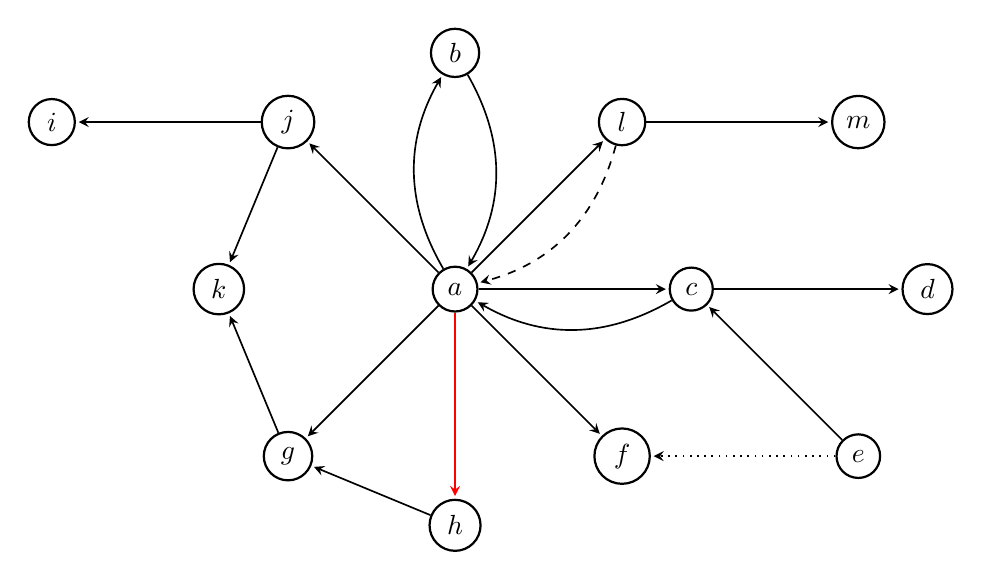
\begin{tikzpicture}[
	> = stealth, % arrow head style
	shorten > = 1pt, % don't touch arrow head to node
	auto,
	node distance = 3cm, % distance between nodes
	semithick % line style
	]
	
	\tikzstyle{every state}=[
	draw = black,
	thick,
	fill = white,
	minimum size = 4mm
	]
	
	\node[state] (a) {$a$};
	\node[state] (b) [above of=a] {$b$};
	\node[state] (c) [right of=a] {$c$};
	\node[state] (f) [below right of=a] {$f$};
	\node[state] (h) [below of=a] {$h$};
	\node[state] (d) [right of=c] {$d$};
	\node[state] (e) [below right of=c] {$e$};
	\node[state] (g) [below left of=a] {$g$};
	\node[state] (j) [above left of=a] {$j$};
	\node[state] (i) [left of=j] {$i$};
	\node[state] (k) [left of=a] {$k$};
	\node[state] (l) [above right of=a] {$l$};
	\node[state] (m) [right of=l] {$m$};

	
	\path[->] (a) edge [bend left] node {} (b);
	\path[->] (b) edge [bend left] node {} (a);
	\path[->] (c) edge [bend left] node {} (a);
	\path[->] (a) edge node {} (c);
	\path[->] (a) edge node {} (f);
	\path[->] (a) edge [red] node {} (h);
	\path[->] (c) edge node {} (d);
	\path[->] (e) edge node {} (c);
	\path[->] (e) edge [dotted] node {} (f);
	\path[->] (a) edge node {} (g);
	\path[->] (a) edge node {} (j);
	\path[->] (j) edge node {} (i);
	\path[->] (h) edge node {} (g);
	\path[->] (j) edge node {} (k);
	\path[->] (g) edge node {} (k);
	\path[->] (l) edge node {} (m);
	\path[->] (a) edge node {} (l);
	\path[->] (l) edge [dashed, bend left] node {} (a);
\end{tikzpicture}

Hier einige Inklusionen, im Bild oben als durchgehende schwarze Pfeile eingezeichnet.

\begin{enumerate}[label = \texttt{ad}]
	\item \blockquote{a. $\implies$ b.}:
	
	Klar!
	
	\item \blockquote{b. $\implies$ a.}:
	
	\begin{enumerate}[label = \arabic*.]
		
		\item Lösung:
		
		Sei $f: \omega \to A$ fast injektiv, d.h.
		
		\begin{align*}
		\Forall x \in f[\omega]:
		|f^{-1}[\Bbraces{x}]| < \infty.
		\end{align*}
		
		Wir fassen $\omega$ und $A$ als Algebren mit leerem Typ auf.
		Auf diese können wir also den Homomorphiesatz anwenden und bekommen eine Abbildung $g$.
		
		\textbf{Achtung!}
		Möglicherweise braucht der Homomorphiesatz das Auswahlaxiom?
		Anstatt einen beliebigen Repräsentanten $u$ von $U$ zu wählen, kann man in unserem Fall den kleinsten $u := \min U$ (von endlich vielen) wählen, um $g(U) := f(u)$ zu definieren.
		Wir haben es schließlich mit Schuhen und nicht mit Socken zu tun!
		
		\phantom{}
		
		\begin{tcolorbox}[standard jigsaw, opacityback = 0]
			\centering
			\includegraphics
			[width = 0.75 \textwidth]
			{Alg/Alg - Satz 2.3.3.16.1 (Homomorphiesatz).png} \\
			\vspace{0.25 cm}
			\includegraphics
			[width = 0.75 \textwidth]
			{Alg/Alg - Satz 2.3.3.16.2 (Homomorphiesatz).png} \\
			\vspace{0.25 cm}
			\includegraphics
			[width = 0.15 \textwidth]
			{Alg/Alg - Satz 2.3.3.16.3 (Homomorphiesatz).png}
		\end{tcolorbox}
		
		\phantom{}
		
		Seien die (unendlich vielen!) Urbilder gemäß ihrem Minimum, vermöge $h$ (strikt monoton steigend), geordnet, d.h.
		
		\begin{align*}
		h := (U_n)_{n \in \omega}:
		\omega \to \omega / \sim:
		\min U_1 < \min U_2 < \cdots
		\end{align*}
		
		$g \circ h: \omega \to A$ ist, als Verkettung injektiver Funktionen, injektiv.
		
		\item Lösung:
		
		Sei $f: \omega \to A$ fast injektiv. \\
		Definiere die injektive Funktion $f': \omega \to A$ durch
		\begin{align*}
		f'(0) &:= f(0) \\
		f'(n) &:= f(\min\{k \in  \N:  f(k) \notin f[\{0,\dots,n-1\}]\}), \quad n \geq 1.
		\end{align*}
		Da das Urbild jedes Bildpunktes endlich ist, exisitiert dieses Minimum immer.
		
	\end{enumerate}

	\item \blockquote{a. $\implies$ c.}: Sei $f: \omega \to A$ injektiv.
	Definiere
	\begin{align*}
	g := \{(f(n),f(n+1)): n \in \omega\} \cup \{(a,a): a \in A \setminus f(\omega)\}
	\end{align*}
	$g$ ist sicher auf ganz $A$ definiert, injektiv und es gilt $f(0) \notin g(A)$.
	
	Diese Implikation wurde auch in Aufgabe 269 gezeigt.
	
	\item \blockquote{c. $\implies$ a.}: Siehe letzte Übung Aufgabe 270.
	
	\item \blockquote{c. $\implies$ d.}:
	
	Klar.
	
	\item \blockquote{e. $\implies$ c.}:
	
	Sei $x \not \in A$ und $f: A \to A \cup \Bbraces{x}$ bijektiv.
	$f^{-1} |_A: A \to A$ ist injektiv, trifft aber nicht $f^{-1}(x)$, ist also nicht surjektiv.
	
	\item \blockquote{a. $\implies$ f.}: Sei $f: \omega \to A$ injektiv. Definiere
	
	\begin{align*}
	g := \{(f(n+1),f(n)): n \in \omega\} \cup \{(a,a): a \in A \setminus f(\omega)\}
	\cup \{(f(0),f(0))\}
	\end{align*}
	$g$ ist surjektiv, aber nicht injektiv.
	
	\item \blockquote{h. $\implies$ g.}:
	
	Klar!
	
	\item \blockquote{a. $\implies$ g.}:
	
	Sei $f: \omega \to A$ injektiv.
	Es gibt folglich also eine (surjektive) Linksinverse $f^{-1}: f[\omega] \to \omega$.
	Wir setzen diese zu einer (surjektiven) Funktion $g: A \to \omega$ beliebig fort.
	
	\item \blockquote{g. $\implies$ k.}:
	
	Sei $f: A \to \omega$ surjektiv.
	
	\begin{gather*}
	g:
	P(A) \to \omega:
	M \mapsto \min f[M],
	\quad
	g_\mathrm{fin} := g |_{P_\mathrm{fin}(A)},
	\quad
	g_\mathrm{sing} := g_\mathrm{fin} |_{P_\mathrm{sing}(A)} \cong f \\
	\implies
	\omega
	\supseteq
	g(P(A))
	\supseteq
	g_\mathrm{fin}(P_\mathrm{fin}(A))
	\supseteq
	g_\mathrm{sing}(P_\mathrm{sing}(A))
	=
	f(A)
	=
	\omega
	\end{gather*}
	
	$g$, $g_\mathrm{fin}$, und $g_\mathrm{sing}$ sind also auch allersamt surjektiv.
	
	\item \blockquote{a. $\implies$ j.}:
	
	Sei $f: \omega \to A$ injektiv, so auch $g: \omega \to P_\mathrm{fin}(A): n \to \Bbraces{n}$.
	
	\item \blockquote{j. $\implies$ i.}:
	
	Klar!
	
	\item \blockquote{j. $\implies$ k.}:
	
	Verwende \blockquote{a. $\implies$ g.} für $P_\mathrm{fin}(A)$ anstelle von $A$.
	
	\item \blockquote{a. $\implies$ l.}:
	
	Wir führen einen Widerspruchsbeweis. Sei also $A$ endlich mit $n \in \omega$ und $f: A \to n$ bijektiv und $g: \omega \to A$ injektiv. Dann ist $h:= g \circ g: \omega \to n$ ebenfalls injektiv. Das kann aber nicht sein, denn wir sehen induktiv, dass
	\begin{align*}
		\forall k \in \omega: \forall \alpha: \omega \to k: \alpha \text{ nicht injektiv. }
	\end{align*}
	Für $k = 0 = \emptyset$ gibt es gar keine Abbildung $\alpha: \omega \to k$, also ist die Aussage klar.
	
	Nehmen wir nun also an, die Aussage gilt bereits für $k \in \omega$. Weiters nehmen wir an, es git eine injektive Funktion $\alpha: \omega \to k + 1$. Wegen der Injektivität gibt es genau ein $l \in \omega$ mit $\alpha(l) = \{k\}$. Nun finden wir die injektive Funktion 
	\begin{align*}
		u: \omega \to \omega: x \mapsto
		\begin{cases}
			x &, \text{falls } x < l \\
			x + 1 &, \text{falls } x \geq l
		\end{cases}.
	\end{align*}
	Nun ist $\beta: \omega \to n: x \mapsto \alpha(u(x))$ eine injektive Funktion. Ein Widerspruch zur Induktionsvoraussetzung. 
	
	\item \blockquote{l. $\implies$ m.}:
	
	Sei also $A$ eine undenliche Menge. Definiere
	\begin{align*}
	\mathfrak{M}:=\Bbraces{X \subseteq A \mid X \text{ endlich }}
	\end{align*}
	und sei $X \in \mathfrak{M}$ beliebig. Die Menge $X$ ist endlich, also gibt es ein $n \in \omega$ und eine Bijektion $f:n \to X$. Da $A$ unendlich ist, kann $f:n \to A$ nicht surjektiv sein also gibt es $y \in A \setminus f[n]$. Nun definiere $Z := X \cup \{y\}$ und
	\begin{align*}
	g:n + 1 \to Z: m \mapsto
	\begin{cases}
	y & ,\text{falls } m = n \\
	f(m) & ,\text{sonst }
	\end{cases}.
	\end{align*}
	Wir sehen, dass $g$ bijektiv ist also $Z$ endlich aber $Z \supsetneq X$, also ist $X$ nicht maximal.
\end{enumerate}




Hier Implikationen die sicher nicht gelten, im Bild oben als rote Pfeile eingezeichnet.

\begin{enumerate}[label = \texttt{ad}]
	\item \blockquote{a. $\implies$ h.}: Wenn $f: A \to \omega$ eine surjektive und fast injektive Abbildung ist, dann können wir $A$ schreiben als
	\begin{align*}
		A = f^{-1}(\omega) = f^{-1}\pbraces{\bigcup_{n \in \omega} \Bbraces{n}} = \bigcup_{n \in \omega} f^{-1}\pbraces{\{n\}}
	\end{align*}
	und da $f^{-1}\pbraces{{n}}$ für jedes $n$ endlich ist wissen wir, dass $A$ höchstens abzählbar unendlich sein kann. Da wir aber schon überabzählbar unendliche Mengen kennen kann diese Inklusion im Allgemeinen nicht gelten. 
\end{enumerate}


Hier Implikationen, für die man (zumindest laut Skriptum) das Auswahlaxiom braucht. Im Graphen oben sind das die strichlierten Pfeile.
\begin{enumerate}[label = \texttt{ad}]
	\item \blockquote{l. $\implies$ a.}:
	
	Laut Satz VI.5.1 im Skriptum braucht man hier das Auswahlaxiom.
\end{enumerate}


Hier noch zusätzliche Implikationen, die sich eigentlich schon aus anderen ergeben.


\begin{enumerate}[label = \texttt{ad}]

  \item \blockquote{e. $\implies$ f.}:

  Sei $x \not \in A$ und $f: A \to A \cup \Bbraces{x}$ bijektiv.
  Sei weiters $y \in A$.
  $g: A \to A$ ist surjektiv, $y$ hat aber die beiden verschiedenen Urbilder $f^{-1}(y) \neq f^{-1}(x)$, weil $x \neq y$, ist also nicht injektiv.

  \begin{align*}
    g:
    A \to A:
    z
    \mapsto
    \begin{cases}
      f(z), & f(z) \in A, \\
      y,    & f(z) = x
    \end{cases}
  \end{align*}
\end{enumerate}



Schließlich noch alte Argumentationen, die womöglich nicht stimmen.

\begin{enumerate}[label = \texttt{ad}]
	\item \blockquote{a. $\implies$ h.}: Sei $f: \omega \to A$ injektiv. Definiere
	\begin{align*}
	g = \{(f(n), n): n \in \omega\} \cup \{(a,0): a \in A \setminus f(\omega)\}.
	\end{align*}
\end{enumerate}

\end{solution}

% --------------------------------------------------------------------------------

\begin{exercise}
Bestimmen Sie die Momente und die Momentenerzeugende für die Laplaceverteilung
mit der Dichte $f(x) = \frac{1}{2}e^{-|x|}$.
\end{exercise}

\begin{solution}

Trivial

\end{solution}

\begin{exercise}
$(X_n)$ sei eine Folge von unabhängigen exponentialverteilten Zufallsvariablen
mit Parameter 1.

\begin{itemize}
  \item[(a)] Bestimmen Sie die Verteilung von $Y_n = \max(X_1,\dots,X_n)$
  \item[(b)] Zeigen Sie, dass $Y_n - \log(n)$ in Verteilung konvergiert und bestimmen Sie die Grenzverteilung (Gumbelverteilung, doppelte Exponentialverteilung).
  \item[(c)] Bestimmen Sie die momentenerzeugende Funktion dieser Verteilung.
\end{itemize}

\end{exercise}

\begin{solution}
  Hier könnte Ihre Werbung stehen!

  \begin{itemize}
    \item[(a)] Wir wählen $x \in \R$ beliebig und berechnen die Verteilungsfunktion in diesem Punkt.

    \begin{multline*}
      F_{Y_n}(x)
      = \P \pbraces{Y_n \leq x}
      = \P \pbraces{X_1, \ldots, X_n \leq x}
      = \P \pbraces{\bigcap_{i=1}^n [X_i \leq x]} \\
      \stackrel{\text{Unabh.}}{=}
        \prod_{i=1}^n \P \pbraces{X_i \leq x}
      = \prod_{i=1}^n F_X(x)
      = \pbraces{1 - \exp(-x)}^n 1_{]0, \infty[}(x).
    \end{multline*}

    \item[(b)] Wir nehmen ein beliebiges $x \in \R$, hoffen, dass es ein Stetigkeitspunkt der Grenzverteilungsfunktion unserer Folge von Verteilungsfunktionen ist und rechnen

    \begin{multline*}
      F_{Y_n - \log(n)}(x)
      = \P \pbraces{Y_n - \log(n) \leq x}
        \P \pbraces{Y_n \leq \log(n) + x}
        \pbraces{1 - \exp(-\pbraces{\log(n) + x})}^n
      1_{]0,\infty[}(\log(n) + x) \\
      = \pbraces{1 + \frac{-\exp(-x)}{n}}^n
        \1_{]0, \infty[}(\log(n) + x)
      \xrightarrow{n \to \infty}
        \exp \pbraces{-\exp(-x)} =: F(x).
    \end{multline*}

    Also gilt

    \begin{align*}
      Y_n - \log(n) \xrightarrow{\text{schwach}} Y \sim F.
    \end{align*}

    \item[(c)] Zuerst sei bemerkt, dass die Dichtefunktion von $Y$ gegeben ist durch die Ableitung der Verteilungsfunktion $F$, also die Form

    \begin{align*}
      f:\R \to \R: x \mapsto \exp(-x) \exp \pbraces{-\exp(-x)}
    \end{align*}

    hat. Wie wir in der Rechnung sehen werden gilt $\Forall t < 1:$

    \begin{align*}
      \E(\exp(Yt))
      & \stackrel{\text{TRAFO}}{=}
        \Int[\R]{\exp(xt)}{\P Y^{-1}(x)}
      = \Int[\R]{\exp(xt) f(x)}{\lambda(x)}
      = \Int[\R]{\exp \pbraces{-\exp(-x)} \exp(-x) \exp(xt)}{\lambda(x)} \\
      & \stackrel{u = \exp(-x)}{=}
        - \Int[\infty][0]{\exp(-u) \exp \pbraces{-\log(u)t}}{\lambda(u)}
      = \Int[\R^+]{\exp(-u) u^{-t}}{\lambda(u)} \\
      & =
        \Int[\R^+]{\exp(-u) u^{(1 - t) - 1}}{\lambda(u)}
      = \Gamma(1 - t).
    \end{align*}
  \end{itemize}
\end{solution}

% --------------------------------------------------------------------------------

\begin{exercise}[280]

Seien $A$ und $B$ Mengen, eventuell mit einer zusätzlichen Struktur
(Vektorraum bzw. partielle Ordnung). Welche der folgenden Familien haben endlichen
Charakter? (Achtung: Bei manchen der folgenden Punkte hängt die Antwotz davon ab,
ob $A$ und/oder $B$ endlich oder gar leer sind.)

\begin{itemize}
  \item Alle Teilmengen von $A$.
  \item Alle unendlichen Teilmengen von $A$.
  \item Alle endlichen Teilmengen von $A$.
  \item Alle partiellen Funktionen von $A$ nach $B$.
  \item Alle partiellen injektiven Funktionen von $A$ nach $B$.
  \item Alle partiellen surjektiven Funktionen von $A$ nach $B$.
  \item Alle partiellen nichtsurjektiven Funktionen von $A$ nach $B$.
  \item Die linear unabhängigen Teilmengen von $A$.
  \item Die linear abhängigen Teilmengen von $A$.
  \item Alle partiellen ordnungserhaltenden Abbildungen von $A$ nach $B$.
  (Das heißt, wenn $f(a), f(a')$ definiert sind, und $a \leq a'$ gilt, dann
  auch $f(a) \leq f(a')$.)
\end{itemize}

\end{exercise}

% --------------------------------------------------------------------------------

\begin{solution}

\phantom{}

\end{solution}

% --------------------------------------------------------------------------------

% --------------------------------------------------------------------------------

\begin{exercise}[281]

Sei $A$ eine endliche Menge mit $n$ Elementen. Sei $W(A)$ die Menge aller $(X, R)$, sodass $X \subseteq A$ ist und $R \subseteq X \times X$ eine lineare Ordnung von $X$ ist.
Sei $\simeq$ die Isomorphierelation auf $W(A)$ und $H(A)$ die Menge aller Äquivalenzklassen.

\begin{enumerate}[label = \alph*.]

  \item Für $A = \Bbraces{1, 2, 3}$:
  Wie viele Elemente hat $W(A)$?
  Geben Sie alle an.
  Wie viele Elemente hat $H(A)$?
  Geben Sie alle an.

  \item Für beliebiges $n$:
  Wie viele Elemente hat $H(A)$?

\end{enumerate}

\end{exercise}

% --------------------------------------------------------------------------------

\begin{solution}

\phantom{}

\begin{comment}

  \begin{enumerate}[label = \alph*.]
    \item
    \begin{align*}
      W(A)
      = \{ 1 \leq 2 \leq 3; 1 \leq 3 \leq 2; 2 \leq 1 \leq 3; 2 \leq 3 \leq 1;
      3 \leq 1 \leq 2; 3 \leq 2 \leq 1\}
    \end{align*}
    Wir können die Elemente aus $W(A)$ in kanonischer Weise mit den
    Permutationen auf der Menge $A = \{1, 2, 3\}$ identifizieren.
    Dabei sind alle linearen Ordnungen vermöge der jeweiligen Permutation
    isomorph,  also hat $H(A)$ genau ein Element.
    \item Ist nicht für alle $n$ $H(A)$ einfach ein-elementig?
  \end{enumerate}

\end{comment}

\begin{enumerate}[label = \alph*.]

  \item $W(A)$ und $H(A)$ sind der unteren Darstellung zu entnehmen.

  \begin{align*}
    \begin{array}{c|c|ccc|ccc|c}
      X & \emptyset & \Bbraces{1} & \Bbraces{2} & \Bbraces{3} & \Bbraces{1, 2} & \Bbraces{1, 3} & \Bbraces{2, 3} & \Bbraces{1, 2, 3} \\
        &           &             &             &             &                &                &                &                   \\
      R &           & 1           & 2           & 3           & 1 2            & 1 3            & 2 3            & 1 2 3             \\
        &           &             &             &             & 2 1            & 3 1            & 3 2            & 1 3 2             \\
        &           &             &             &             &                &                &                & 2 1 3             \\
        &           &             &             &             &                &                &                & 2 3 1             \\
        &           &             &             &             &                &                &                & 3 1 2             \\
        &           &             &             &             &                &                &                & 3 2 1             \\
    \end{array}
  \end{align*}

  \item $|H(A)| = n + 1$

\end{enumerate}

\end{solution}

% --------------------------------------------------------------------------------


\end{document}
